\documentclass[aps, prc, reprint, amsmath, groupedaddress, nofootinbib]{revtex4-1}
%\usepackage[compat=1.1.0]{tikz-feynman}
\usepackage[utf8]{inputenc}
\usepackage{hyperref}
\usepackage{amsmath}
\usepackage{amssymb}
\usepackage{amsfonts}
\usepackage{tabularx}
\usepackage{booktabs}
\usepackage{graphicx}
\usepackage{color}
\usepackage{multirow}
\usepackage{verbatim}
\usepackage[inline]{enumitem}
\graphicspath{{fig/}}
\definecolor{theblue}{RGB}{0,50,230}
\usepackage{appendix}
\hypersetup{
  colorlinks=true,
  linkcolor=theblue,
  citecolor=theblue,
  urlcolor=theblue
} 
\usepackage[most]{tcolorbox}

\begin{abstract}
Hard probes created in perturbative processes are excellent probes for the study of the hot and dense QCD matter created in relativistic heavy-ion collisions.
Transport approach, allowing for a coupling to an evolving medium with a fluctuating initial condition, has become a powerful tool in this endeavor. 
However, the implementation of the Landau-Pomeranchuk-Migdal (LPM) effect for medium-induced parton bremsstrahlung and pair production, poses a challenge to semi-classical models: the widely used Boltzmann-type transport equations.  
In this work, we investigated a possible solution to approximate the LPM effect in a ``modified Boltzmann transport" approach, including a prescription for the running coupling constant.
By fixing a numerical parameter, this approach quantitatively reproduces the rates of medium-induced parton splitting predicted by the next-to-lead-log solution of the AMY equation which is valid in the deep-LPM regime of an infinite medium.
We also found a qualitative agreement of our implementation with calculations in a finite and expanding medium, but future improvements are needed for precision at small path length.
This work benefits transport model based studies and the usage of these models in the phenomenological extraction of the jet transport coefficient.


\end{abstract}

\begin{document}
\title{A modified-Boltzmann approach for modeling the hot QCD medium-induce splitting vertices in the deep LPM region}
\author{Weiyao Ke}
\author{Yingru Xu}
\author{Steffen A.\ Bass}
\affiliation{Department of Physics, Duke University, Durham, NC 27708-0305}
\date{\today}
\maketitle 

\section{Introduction}
The study of hard probes in relativistic heavy-ion collisions is moving towards the precision era thanks to upcoming experimental upgrades \cite{ATLAS-Collaboration:2012iwa,Abelevetal:2014dna,STAR:upgrade-hf,Adare:2015kwa,CMS:2017dec} as well as theoretical and computational advances that allow for the execution of jet propagations in a realistic Quark-Gluon-Plasma (QGP) medium (including event-by-event fluctuating initial conditions and temperature-dependent transport coefficients) \cite{Wang:1994fx,Zakharov:1996fv,Baier:1996sk,Zakharov:1997uu,Arnold:2002zm,Gyulassy:2003mc,Kovner:2003zj,Jeon:2003gi,CasalderreySolana:2007pr,Djordjevic:2008iz,Bass:2008rv,Schenke:2009gb,Majumder:2009zu,Majumder:2010qh,Armesto:2011ht,Zapp:2011ya,Ovanesyan:2011xy,Kang:2014xsa,Cao:2016gvr,Kauder:2018cdt,Cao:2017zih}. Among the goals for this research is the characterization of the QGP medium in terms of its jet transport coefficients $\hat{q}$.

Transport models are powerful tools where hard probes can be coupled to the realistic time evolution of the medium with an event-by-event fluctuating initial condition. 
However, the numerical implementation of the QCD analog of the Landau-Pomeranchuk-Migdal (LPM) effect, poses a serious challenge to a class of widely used models: the Boltzmann-type transport equation, including the Langevin dynamics.
In a dense medium, multiple scatterings act coherently within the formation time ($\tau_f$) of the medium-induced parton splitting \cite{PhysRev.103.1811,Wang:1994fx,Zakharov:1996fv,Zakharov:1997uu,Baier:1996kr,Baier:1996sk}.
The resultant bremsstrahlung rate differs from those estimated assuming independent incoherent) collisions.
As a result, bremsstrahlung in a medium becomes an effectively $n$-body to $(n+1)$-body process with a finite extend $\tau_f$ in space-time compare. At high energy, $\tau_f$ can be much larger than collisional mean-free-path $\lambda_{\textrm{el}}$, and can be comparable to the typical inverse gradient of the macroscopic quantities of the medium created in heavy-ion collisions.
These situations are particularly difficult to treat in a Boltzmann transport equation with local and few-body collision terms. 
To simplify the parton bremsstrahlung while retaining essential qualitative features, different approximations and perscriptions are used to incoporate the LPM effect into transport models \cite{Cao:2013ita,ColemanSmith:2012vr,Xu:2004mz,Zapp:2011ya,Gossiaux:2012cv,Park:thesis}.
These models are then applied to phenomenological studies and used for physical parameter extraction such as $\hat{q}$.
However, there has not been sufficient attention to the quantitative comparisons of these approximate implementations to the theoretical calculations.
Such a step is essential for a reliable extraction of the jet transport properties.

In this work, we have developed an approximation scheme for the inclusion of LPM effect into the transport model, aiming for quantitative comparison between the model and the theory.
The resultant technique is hereafter termed as ``the modified Boltzmann transport" approach.
Here we give a short overview of the approach. 
The semi-classical transport model propagates the hard partons inside a quark-gluon plasma, under the influence of both elastic collisions with the medium, as well as incoherent parton bremsstrahlung (inelastic processes) from independent collisions.
We first focus on the simplest scenario of hard parton propagating in an infinite medium with a constant temperature.
The LPM effect is implemented as a modification to the incoherent inelastic rates, where elastic collisions broaden the transverse momentum between the outgoing hard partons and the incoherent rate is reduced by a factor $P$.
The suppression probability $P$ is obtained from the leading-log (LL) approximation of parton splitting when the number of coherent collisions is large $N_{\textrm{coh}} = \tau_f/\lambda_{el} \gg 1$ (the deep-LPM region), and $P \propto \lambda_{el}/\tau_f$.
Moreover, a quantitative agreement with the theory can be achieved by introducing a next-to-lead-log (NLL) correction to $P$.
The modified transport model describes the rates for in-medium bremsstrahlung $q\rightarrow q+g$, $g\rightarrow g+g$, and pair production $g\rightarrow q+\bar{q}$ surprisingly well in the deep-LPM region.
Next, we apply the model to cases beyond an infinite and static medium, because the realistic medium created in heavy-ion collisions is finite, fluctuating, with a fast dropping temperature profile due to the violent expansion. 
It is true that the current approach is developed by matching to theoretical calculations in the deep LPM region assuming many coherent collisions, but for a thin medium, the role of the interference pattern between only a few coherent collisions becomes important.
In principle, one should resort to other techniques such as the opacity expansion \cite{Wiedemann:2000za,Gyulassy:1999zd} for computation a thin medium. 
Nevertheless, we do find the current method qualitatively reproduces the theroretical calcualtions of path-length dependence \cite{CaronHuot:2010bp} and the medium expansion rate depedence \cite{Baier:1998yf} of the radiation rates.

Finally, we find it instructive to compare the current method to two other Monte Carlo implementations of the medium-induced radiation processes that have been used in previous studies.
We found subtle differences in the construction of these models can lead to incorrect implementation of the LPM effect or introduce correlations between sequential bremsstrahlung partons that is beyond the leading-order theory used for the model.
We want to draw attention on the phenomenological consequences of these differences. 
Especially, these differences affect the interpretation of the extracted physical parameters such as in-medium coupling and $\hat{q}$.
This also demonstrates the importance of making direct comparison between the transport model and theoretical calculations as practiced in this work.

This paper is organized as follows. 
Section \ref{section:Boltzmann} introduces the ingredients of the semi-classical transport model that is to be modified.
In section \ref{section:modified-Boltzmann}, we propose the modifications to the aforementioned model in Section \ref{section:Boltzmann} to include the LPM effect.
In section \ref{section:results} and appendix \ref{app:tune-spectrum}, we provide detailed comparisons between the simulation and the NLL solution in the deep-LPM regime.
Effects of a finite and expanding medium are investigated in section \ref{section:more}.
In section \ref{section:compare}, we compare this work to two previously used Monte-Carlo implementations of the LPM effect in transport models.
Finally, section \ref{section:summary} summarizes and discusses the future applications of the model.



\section{Semi-classical transport approach with incoherent rates}\label{section:Boltzmann}
In this section, we construct the transport model assuming collisions are independent and will discuss in great detail in the next section on the inclusion of the LPM effect.
Focusing on hard partons, the collisions are categorized into elastic (hard particle number conserving) and inelastic processes (hard particle number non-conserving). 
The inelastic processes are further divided into parton-splitting and parton-merging contribution. 
The Boltzmann equation relates evolution of the hard parton distribution function $f_H$ to these collision processes,
\begin{eqnarray}
\frac{df_H}{dt} = \mathcal{C}_{\textrm{el}}[f_H] + \mathcal{C}_{\textrm{inel}}[f_H].
\end{eqnarray}
As a remark, we have suppressed writing the dependence of the collision term on the light parton distribution functions, because we assume them to be the thermal equilibrium ones with Boltzmann statistics $f_0(p) = e^{-p\cdot u/T}$. 
And $T$ and $u$ are the medium temperature and four-velocity that can be obtained from a medium evolution model. 
We also neglects the collisions between two or more hard partons and the back reaction from hard parton to the medium due to their small population  in actual high energy nuclear collisions.
As a result, the above Boltzmann equation is linearized with respect to $f_H$.

A linearized Boltzmann equation can be solved using a collision rate approach.
First, hard partons are represented by $\delta$-functions in the phase space $f_H(t,\mathbf{x},\mathbf{p}) \approx \sum \delta^{(3)}(\mathbf{p}-\mathbf{p}(t))\delta^{(3)}(\mathbf{x}-\mathbf{x}(t))$.
Each particle travels in a straight line and occasionally its momentum changes drastically due to collisions.
This way, one obtains a stochastic solution of the time evolution of $f_H$.
The collision probability per unit time (i.e., the collision rate) is 
\begin{eqnarray}
R = \frac{g_i}{2E_1}\int  \frac{d^3p_2}{2E_2(2\pi)^3} f_0(p_2)2\hat{s} \sum_i \int_{-\hat{s}}^{0}\frac{d\sigma_i}{d\hat{t}}d\hat{t}.
\label{eq:incoh_rate}
\end{eqnarray}
For simplicity, we have only shown the case that the hard parton with momentum $p_1$ collides with one medium parton with momentum $p_2$.
$\hat{s}, \hat{t}$ are the Mandelstam variables of the two-body collisions. 
$d\sigma_i/d\hat{t}$ is the differential cross-sections of channel $i$, including both elastic and inelastic contributions.

The in-medium cross-sections $d\sigma_i$ are dominated by $\hat{t}$ channel processes which diverges like $1/\hat{t}^2$ in the vacuum.
In a medium, screening effects regulates the cross-section and make finite the physical quantities; however, the cross-section becomes complicated and its form depends the choice of reference frame.
Here, we borrow an elegant solution from \cite{Ghiglieri:2015ala} to separate the in-medium collisions depending on the momentum transfer-$q$ between the hard parton and the medium.
The large-$q$ transfer (hard) scattering rate uses cross-sections computed in the vacuum, because the medium modification to these hard modes is small.
The associated rates are obtained from equation \ref{eq:incoh_rate} while restricting $q$ to be larger than a switching scale $Q_{\textrm{cut}}$.
The small-$q$ transfer processes are frequent and soft, which allows a diffusion approximation of its effect on the trajectory of the hard parton,
\begin{eqnarray}
\mathbf{x}(t+\Delta t) &=& \frac{\mathbf{p}}{E}\Delta t\\
\mathbf{p}(t+\Delta t) &=& \mathbf{p} - \eta_{D,S} \mathbf{p} \Delta t + \mathbf{\xi}(t) \Delta t
\end{eqnarray}
The effect of the soft-interaction are absorbed into the drag coefficients $\eta_d$, and the covariance of the thermal random force $\mathbf{\xi}$,
\begin{eqnarray}
\left\langle\xi_i(t)\xi_j(0)\right\rangle = \delta(t) \left(
\frac{p_i p_j}{p^2}\hat{q}_{L,S} + \left(
\delta_{ij}-\frac{p_i p_j}{p^2}
\right)\frac{\hat{q}_S}{2} 
\right)
\end{eqnarray}
Here, the subscript ``$S$'' reminds us that these numbers should only contain soft contributions with $q<Q_{\textrm{cut}}$.
The switching scale $Q_{\textrm{cut}}$ is chosen to be greater than the Debye screening mass $m_D$,
\begin{eqnarray}
m_D^2 = \frac{4\pi \alpha_s}{3}\left(N_c+\frac{N_f}{2}\right) T^2.
\end{eqnarray}
One of the many advantages of this separation is avoiding the complicated in-medium propagators, while still achieve an leading order accuracy with a reasonable choice of $Q_{\textrm{cut}}$ at weak coupling as shown in \cite{Ghiglieri:2015ala}.

\paragraph{Elastic processes} The two-body matrix-elements in vacuum that enters the large-$q$ collisions rates can be found in standard literature \cite{RevModPhys.59.465}.
For small-$q$ diffusion sector, the transverse and longitudinal momentum diffusion coefficients $\hat{q}_S, \hat{q}_{S,L}$ in a weakly coupled theory have been calculated in \cite{Ghiglieri:2015ala} at leading order,
\begin{eqnarray}
\hat{q}_S = \int_0^{Q_{\textrm{cut}}^2} dq^2 \frac{\alpha_s m_D^2 T}{q^2 (q^2+m_D^2)},
\label{eq:qS} \\
\hat{q}_{S,L} = \int_0^{Q_{\textrm{cut}}^2} dq^2 \frac{\alpha_s m_\infty^2 T}{q^2 (q^2+m_\infty^2)}.
\label{eq:qSL}
\end{eqnarray}
$m_{\infty}$ is the asymptotic gluon thermal mass $m_{\infty}^2 = m_D^2/2$.
Finally, the drag coefficient is determined by the Einstein relation between the transport coefficients,
\begin{eqnarray}
\eta_{D,S} = \frac{\hat{q}_{L,S}}{2ET} - \frac{d\hat{q}_{L,S}}{dp^2} - \frac{\hat{q}_{L,S} - \hat{q}_S/2}{p^2}.
\end{eqnarray}

\paragraph{Inelastic processes} The inelastic collision term is also separated into a large-$q$ $2\leftrightarrow 3$ body inelastic collision rate plus an effective $1\leftrightarrow 2$ body diffusion-induced parton splitting / jointing rate.
The matrix-elements of $2\leftrightarrow 3$ body collisions are derived under the limit $k_\perp^2, q_\perp^2 \ll x(1-x)\sqrt{\hat{s}}$.
Here, $x$ is the light-cone energy fraction of the initial state hard parton carried by one of the final state hard parton, $q_\perp$ is the transverse component of $q$ in the center-of-mass frame of the collision, and $k_\perp$ is the transverse momentum of between the two split hard partons in the final state. 
A list of these matrix-elements can be found in appendix \ref{app:23}.
Again, the rates are obtained from equation \ref{eq:incoh_rate} imposing $q>Q_{\textrm{cut}}$.

The diffusion-induced splitting rate uses the restriction $q<Q_{\textrm{cut}}$ in equation \ref{eq:incoh_rate}, and uses the limit $q_\perp \ll k_\perp$ of the $2\rightarrow 3$  matrix-elements listed in appendix \ref{app:23},
\begin{eqnarray}
R_{1\rightarrow 2} &=& \frac{g_i}{2E_1}\int  \frac{d^3p_2f_0(p_2)}{2E_2(2\pi)^3} 2\hat{s} \int_{0}^{Q_{\textrm{cut}}^2} q_\perp^2 \frac{d\sigma_{\textrm{el}}}{q^2} dq^2\\\nonumber
&& \times \int d k_\perp^2 dx \frac{\alpha_s P(x) }{2\pi (k_\perp^2 + m_\infty^2)^2} \label{eq:rate12-1}
\end{eqnarray}
where $m_\infty$ is added to screen the divergence and $P(x)$ is the vacuum splitting function listed in appendix \ref{app:23}.
Now, one may notice that the first line in \ref{eq:rate12}, upon summing over all channels, simply computes the average transverse momentum received by the hard parton per unit time from soft interactions below the momentum cut-off $Q_{\textrm{cut}}$.
So we can rewrite $R_{1\rightarrow 2}$ using the soft transport coefficients $\hat{q}_{S}$,
\begin{eqnarray}
R_{1\rightarrow 2} &=& \hat{q}_S\int d k_\perp^2 dx \frac{\alpha_s P(x) }{2\pi (k_\perp^2 + m_\infty^2)^2} \label{eq:rate12-2},
\end{eqnarray}
which is our final expression for the diffusion induced inelastic collision rate for the incoherent transport equation.
Finally, the collision rates of the reverse processes $3\rightarrow 2$ and $2\rightarrow 1$ processes can be written down by the requirement of detailed balance.

\paragraph{The transport equation in the incoherent limit}
Combining all these processes, we summarize the transport equation with independent collisions into
\begin{eqnarray}
\frac{df}{dt} = \mathcal{D}[f] + \mathcal{C}_{1\leftrightarrow 2}[f] + \mathcal{C}_{2\leftrightarrow 2}[f] + \mathcal{C}_{2\leftrightarrow 3}[f].
\end{eqnarray}
The distribution function of the hard parton evolves under the effect of diffusion $\mathcal{D}$, large-$q$ elastic collision $\mathcal{C}_{2\leftrightarrow 2}$,  diffusion induced parton splitting / merging $\mathcal{C}_{1\leftrightarrow 2}$, and large-$q$ inelastic collisions $\mathcal{C}_{2\leftrightarrow 3}$. 


\section{Modeling LPM effect by a modified transport simulation}\label{section:modified-Boltzmann}
The incoherent transport equation only works for a small window of phase-space where the formation time of the splitting processes is small compared to elastic-mean-free path, which is not the case for energetic splittings and we expect a modification to the above transport approach in this region.

From uncertainty principal, the splitting formation time can be obtained as the inverse of the difference between the final-state energy and the initial-state energy of the splitting system,
\begin{eqnarray}
\tau_f^{-1} \sim \delta E = \frac{[(1-x)\vec{k}_\perp - x\vec{q}_\perp]^2}{2x(1-x)E} 
\label{eq:tauf}
\end{eqnarray}
In the reference frame where the initial parton moves in the $z$-direction, the formation time becomes $\tau_f = 2x(1-x)E/k_\perp^2$.
For high energy splitting, such a formation time can be very large compared to the mean-free-path $\lambda \sim 1/g^2T$ from leading order estimation.
Therefore, the transverse momentum $k_\perp$ can be broadened by multiple scatterings during $\tau_f$.
In an infinite medium, when the number of multiple scatterings $N$ is large (the deep-LPM region), one has on average
\begin{eqnarray}
\left\langle k_\perp^2 \right\rangle \approx \hat{q} \tau_f \label{eq:broaden}
\end{eqnarray}
where $\hat{q} = d \left\langle k_\perp^2 \right\rangle / dt$ is the transport coefficient with contributions from all types of interaction.
Combining Eq. \ref{eq:tauf} and Eq. \ref{eq:broaden}, a crude estimate for the average formation time in an infinite medium is then $\left\langle \tau_f \right\rangle \sim \sqrt{2x(1-x)E/\hat{q}}$.
The multiple interactions within the time has to be resumed and in the leading $\ln(N)$ (leading-logarithmic), the transition rate from interacting with $N$ coherent scattering centers is effectively reduced to the rate induced by with one scattering center. 
The LPM effect strongly modifies the radiation spectrum with a factor $\lambda/\tau_f \sim \sqrt{T/(x(1-x)E)}$ for $\omega, E-\omega \gg T$, where $\omega = xE$ is the energy of the radiated daugther parton.
One also sees that the region where the incoherent transport model is valid is limited to $\lambda \gg \tau_f$, or $\omega, E-\omega \ll T$.
Therefore, quite fundamental modification has to be made to the Boltzmann equation to include splitting processes properly which we shall refer as the so-called ``modified Boltzmann transport" approach.

\subsection{An ansatz for the modified transport}
We start by investigating the leading-order calculation of medium-induced parton splitting in a ``brick" and identify the modification to the Botlzmann formulation.
Here we quote the reorganized formula for medium-induced splitting from \cite{CaronHuot:2010bp},
\begin{eqnarray}
\frac{dP^{a}_{bc}}{d\omega} &=& \int_0^\infty dt \frac{g^2}{\pi E} P_{bc}^{a(0)}(x) \int_t^\infty dt'  F(t', t)
\label{eq:full-theory}
\\
F(t', t) &=& \mathfrak{Re} \int_{{\bf q}', {\bf q}} \frac{i {\bf q}'\cdot {\bf q}}{\delta E} \mathcal{C}(t') K(t', {\bf q}'; t, {\bf q})
\end{eqnarray}
where $P_{bc}^{a(0)}$ is the vacuum splitting function and $\delta E$ is the light-cone energy difference between initial and final states. 
The $\mathcal{C}(t')$ operator is a Boltzmann-type collision operator such that,
\begin{eqnarray}
\mathcal{C}[f] = \int_{\bf q} g^2\mathcal{A}(q_\perp^2)
&&\left\{  \frac{C_b+C_c-C_a}{2}\left(f_{\bf p}-f_{{\bf p}-{\bf q}}\right) \right.\\\nonumber
 +&&    \frac{C_a+C_c-C_b}{2}\left(f_{\bf p}-f_{{\bf p}+x{\bf q}}\right) \\\nonumber
+&&  \left. \frac{C_a+C_b-C_c}{2}\left(f_{\bf p}-f_{{\bf p}+(1-x){\bf q}}\right)\right\},
\end{eqnarray}
where $C_i$ is the color factor of each parton and $\int_q = \int dq^2/(2\pi)^2$.
The collision kernel is given by \cite{Aurenche:2002pd},
\begin{eqnarray}
\mathcal{A}(q_\perp^2) = \frac{m_D^2 T}{q^2\left(m_D^2+q^2\right)}
\end{eqnarray}
Finally, $K(t', {\bf q}'; t, {\bf q})$ is the propagator of the transverse  Hamiltonian $\hat{H} = \delta E - i\mathcal{C}$ in the momentum representation.
This rather compact result is actually hard to implement in a Boltzmann formulation, because of the double time integral that signatures the quantum transition.
Moreover, the branching probability generally dependents on the temperature and flow velocity profiles of the medium, making it a computationally heavy task when coupled to dynamical evolving and fluctuating medium.

Our approximation towards a modified Boltzmann transport formulation starts by replacing the effect of the temporal correlator $F(t',t)$ with a simple ansatz,
\begin{eqnarray}
F(t', t) \rightarrow \frac{1}{N}\sum_{i=1}^N \frac{b}{\tau_i(t)} \delta(t-t'- a \tau_i(t))
\label{eq:ansatz}
\end{eqnarray}
Here the function $F(t', t)$ is approximated by an ensemble of $N$ independent copies of the branching system $a\rightarrow b+c$.
These copies are generated according to the incoherent inelastic rates of the $1\rightarrow 2$ and $2\rightarrow 3$ processes.
Each copy ``$i$" evolves with the influence of the elastic broadening, and there is certain probability for this copy to have a formation time $\tau_i$ at time $t$ during the evolution.
The delta function imposes that the branching that starts at time $t'$  is thought to be formed at time $t+a\tau_f$.
The additional factor $b/\tau_f$ corrects for that the probability for the actually branching is suppressed compared to the incoherent probability, as guided by the leading-log picture.
This ansatz of representing the function $F(t', t)$ with information at $t$ and $t'$ of an ensemble of particles follows the same spirit of the Monte-Carlo solver of the traditional Boltzmann equation, where the distribution function is represented by an ensemble of particles at time $t$.
Of course, this is only a crude ansatz for the overall effect of $F(t', t)$ as the latter is actually highly oscillating, and the validity has to be examined by comparing its prediction with the theoretical calculations.
Finally, $a$ and $b$ are dimensionless factors whose forms shall be determined later and will be tuned to achieve an optimal level of agreement to theoretical calculations.

With such an ansatz, the medium-induced splitting probability reduces to,
\begin{eqnarray}
\nonumber
\frac{dP^{a}_{bc}}{d\omega} &=& \int_0^\infty dt \frac{g^2 P_{bc}^{a(0)}}{\pi E\tilde{\lambda}(t)} \frac{1}{N}\sum_{i=1}^N\\\nonumber
&&\times \int_t^\infty dt' \frac{b \tilde{\lambda}(t)}{\tau_i(t)} \delta(t-t'- a \tau_i(t)) \\
&=& \frac{1}{N}\sum_{i=1}^N\int_0^\infty dt \frac{dR_{\textrm{incoh}}(t)}{d\omega} \times \left.\frac{ab\tilde{\lambda}(t)}{\tau_f(t',t)}\right|_{t'=t+a\tau_f}
\label{eq:procedure}
\end{eqnarray}
where we have divided and multiplied back an effective mean-free-path $\tilde{\lambda}(t) = m_D^2/\hat{q}_g$ so that we may interpret the quantity immediately after the $dt$ integral as the incoherent splitting rate $R_{\textrm{incoh}}$.
The reason of using an effective $\tilde{\lambda}$ is because it can be defined for both scattering and diffusion process, provided only screening mass and the transverse transport parameter of that process.
From equation \ref{eq:procedure}, it is clear how we can modify the standard Boltzmann transport to approximately include the LPM effect in the leading-log picture,
\begin{enumerate}
\item Evolve each parton by solving the collision rate equation with incoherent rate from $t$ to $t+\Delta t$.
\item The daughter partons from splittings are not immediately treated as independent (``preformed"). They are evolved together with the mother parton. Preformed partons only undergoes elastic collisions (the mother parton can keep creating more copies of splittings through incoherent inelastic processes).
\item Recalculate formation time $\tau_f$ after each time step.
\item Repeat steps 1 to 3 until $t' > t + a\tau_f$ is satisfied. 
\item Accept this splitting copy with probability 
\begin{eqnarray}
p = \min\left\{1, \frac{ab\tilde{\lambda}(t)}{\tau_f}\right\}
\label{eq:rejection}
\end{eqnarray}
Daughter partons of accepted splittings will be treated as independent objects from time $t'$, and will interact through both elastic and inelastic channels.
Rejected splittings are dropped and do not cause any physical effect.
\end{enumerate} 
A key step is a self-consistent determination of the formation time as described in step 4, which in a static medium, results in an averaged formation time  that scales like $\left\langle\tau_f\right\rangle \propto \sqrt{2x(1-x)E/\hat{q}}$.
This procedure also generalizes to medium with evolving temperature profile, as the elastic broadening can be performed along with the time evolution of the medium.
This iterative procedure was first developed and implemented by \cite{Zapp:2011ya}.

Such an ansatz only captures the qualitative behavior of the LPM effect in the leading-log picture. 
To make it more useful, we compare it to an next-to-leading-log calculation in an infinite medium in the following subsection and determine the forms of $a$ and $b$.

\subsection{Matching the ansatz to theoretical calculation in an infinite medium in the deep-LPM region}
Going to an infinitely large medium with an uniform temperature, equation \ref{eq:full-theory} can be cast into its asympototic form known as the AMY formalisim \cite{Arnold:2002ja,Arnold:2002zm,Arnold:2003zc},
\begin{eqnarray}\label{eq:AMY-1}
\frac{dP^a_{bc}}{dt dx} &=& \frac{1}{2E\nu_a} \frac{\alpha_s d_a P^{a(0)}_{bc}(x)}{2x^2(1-x)^2}\int\frac{d^2\vec{h}}{(2\pi)^2}2\vec{h}\cdot \mathfrak{Re} \vec{F}
\end{eqnarray}
where we have dropped the Bose enhancement and the Pauli blocking factors from the original formula.
The vector-valued function $\vec{F}(\vec{h}; p, x)$ satisfies the following static equation,
\begin{eqnarray}\label{eq:AMY-2}
2\vec{h} &=& i\frac{h^2 \vec{F}(\vec{h})}{p^3 2x(1-x)} + g^2 \mathcal{C}[\vec{F}]
\end{eqnarray} 
The exact solution can be solved numerically and has already been applied to transport study \cite{Jeon:2003gi,Schenke:2009gb}, but we shall use an approximated semi-analytic solutions obtained by the author of \cite{Arnold:2008zu}.
These approximated solutions were obtained at the leading-log (LL) and next-to-leading-log (NLL)accuracy, and the NLL solution was shown to be a good approximation of the numerical results in the deep LPM regime $\omega \gg T$.

At leading-log order, a small-$q$ expansion was performed to obtained a diffusion approximation to the operator $\mathcal{C}$ below a certain cut-off $q<Q_0$.
The resulting leading-log solution is \cite{Arnold:2008zu},
\begin{eqnarray}\label{eq:AMY-LL}
\frac{dP_{bc}^{a,\textrm{LL}}}{dt dx} &=& \frac{\alpha_s P_{bc}^{a(0)}}{\pi\sqrt{2}}
\sqrt{\frac{\hat{q}_3(x, Q_0^2)}{2x(1-x)E}}
\end{eqnarray}
Where the $\hat{q}_3$ is defined as an effective transport parameter for conveniences,
\begin{eqnarray}
\hat{q}_3(x, Q_0^2) &=& \alpha_s T m_D^2 \ln\left(1+\frac{Q_0^2}{m_D^2}\right) C_{abc}(x),\label{eq:qhat3}
\end{eqnarray}
depending on the colors of the partons,
\begin{eqnarray}
C_{abc}(x) &=&  \frac{C_b+C_c-C_a}{2} + x^2 \frac{C_a+C_c-C_b}{2} \\\nonumber
&+& (1-x)^2\frac{C_a+C_b-C_c}{2}
\end{eqnarray}
Comparing the leading-log formula to the modified Boltzmann approach in equation \ref{eq:procedure} and the rejection probability of the incoherent branchings in equation \ref{eq:rejection}, there is indeed a piece in equation \ref{eq:AMY-LL} that plays the row of the inverse formation time $\langle\tau_f^{-1}\rangle \sim \sqrt{\hat{q}_3 / 2x(1-x)E}$.
We can also insert an $1/\lambda \times \lambda$ into equation \ref{eq:rejection} so that it looks more familiar like equation \ref{eq:procedure}.
However, the effective $\hat{q}_3$ is differed by an $x$-dependent color factor $C_{abc}$ from the elastic broadening expected from the rescattering of only one daughter parton that is implemented in our algorithm.
This can be improved by defining a process- and $x$-dependent $a$ parameter in equation \ref{eq:ansatz},
\begin{eqnarray}
a \rightarrow a_{abc}(x) = \frac{C_A}{C_{abc}(x)}
\end{eqnarray}

From equation \ref{eq:AMY-LL}, the LL solution is still ambiguous upto an unknown cut-off $Q_0$ through $\hat{q}_3(x, Q_0^2)$.
This logarithmic dependence on $Q_0$ of $\hat{q}_3$ in equation \ref{eq:qhat3} comes from integrating the perturbative tail of the collision kernel $\int \mathcal{A}(q^2) q^2 dq^2$ when the cut-off scale $Q_0^2 \gg m_D^2$.
This $Q_0$ ambiguity can be improved by going to the NLL order, where the contribution of the collision kernel above $Q_0$ is treated as a pertrubation on top of the LL solution.
This ``hard" correction to the ``multiple-soft" approximation is also recently studied in \cite{Mehtar-Tani:2019tvy} in the BDMPS framework.
In both works, the NLL result is expressed as the LL solution with the unknown $Q_0$ replaced by $Q_1$,
\begin{eqnarray}
Q_1^2  \approx \sqrt{\omega \hat{q}} \approx \sqrt{\omega \alpha_s C_R m_D^2 T \ln\frac{Q_0^2}{m_D^2}}
\label{eq:Q1}
\end{eqnarray}
or one can uses a self-consistent determination of $Q_1$ as in \cite{Arnold:2008zu} to eliminated the dependence of $Q_0$ from the formula,
\begin{eqnarray}
Q_1^2 &=& \sqrt{2 x (1-x) E \alpha_s T m_D^2}\\\nonumber
&\times & \left(
\frac{C_b+C_c-C_a}{2}\ln\frac{2\xi Q_1^2}{m_D^2} \right.\\\nonumber 
&+& \frac{C_a+C_c-C_b}{2} x^2 \ln\frac{2\xi Q_1^2}{x^2 m_D^2} \\\nonumber 
&+& \left.\frac{C_a+C_b-C_c}{2} (1-x)^2 \ln\frac{2\xi Q_1^2}{(1-x)^2 m_D^2} \right)^{1/2}
\label{eq:Q1-sf}
\end{eqnarray}
Therefore, the reasonable choice of the scale in $\hat{q}_3$ is of similar order as the transverse momentum of the branching $k_\perp^2 \approx \sqrt{\omega \hat{q}}$.
Now, checking what this scale is in the original transport approach: the large-$Q$ two-body matrix-element in equation \ref{eq:incoh_rate} is always integrated upto the maximum transfer bounded by the center-of-mass energy $\sqrt{\hat{s}}$ of each individual collision. 
Ignore the slow $\hat{s}$-dependence of the elastic cross-section at high-energy and average over the medium parton momentum $p_2$ in $\hat{s} = (p+p_2)^2$ over the thermal distribution, then the average $Q_{0}^2 \sim \langle\hat{s}\rangle = 6ET$ in the incoherent simulation.

We must correct of this difference in scale; otherwise, the ansatz with an native choice of upper limit of the matrix-element integration leads to systematically deviation from the NLL solution in a logarithmic manner.
The correction can be achieved by using a scale-dependent $b$ parameter,
\begin{eqnarray}
b &=& 0.75\sqrt{\frac{\ln(\hat{Q}_1^2 )}{\ln(\hat{Q}_0^2 )}}.
\label{eq:NLL-b}
\end{eqnarray}
with $\hat{Q}_1^2$ and $\hat{Q}_0^2$ given by,
\begin{eqnarray}
\hat{Q}_1^2 &=& 1 + \frac{\sqrt{2x(1-x)E\hat{q}}}{m_D^2} \approx 1 + \frac{\tau_{f,i}}{\tilde{\lambda}}, \\ 
\hat{Q}_0^2 &=& 1 + \frac{6ET}{m_D^2}.
\end{eqnarray}
The prefactor $0.75$ is the only numerical constant that we have tuned when we compared the modified Boltzmann simulation to the NLL solutions in the next section, and it be the same throughout the rest of the paper.

As a remark, this logarithmic correction comes from the $\mathcal{A}(q^2) q^2 dq^2 \sim dq^2 /q^2$ integration of the collision kernel at large-$q^2$.
Therefore, if one assumes and implements certain collision kernel that vanishes sufficiently fast at large-$q$, this logarithm factor in $b$ should be dropped. 

\subsection{Agreement in the the the Bethe-Heitler region when $Q^2$ is large}
In the previous subsection, we have shown how the modified Boltzmann transport approach can be matched to the NLL solution in the deep-LPM region where $\tau_f \gg \lambda_{\textrm{el}}$.
There is actually another region of phase-space of the inelastic processes where the transport method agrees with the theoretical calculation.
This is the large $Q^2 > Q_{\textrm{cut}}^2 \gg m_D^2$ region in the Bethe-Heitler regime $\tau_f \ll \lambda_{\textrm{el}}$.
One can see from the rejection probability \ref{eq:rejection} that the modified Boltzmann method goes back to the original Boltzmann equation when $\lambda_{\textrm{el}}/\tau_f\gg 1$.
We will briefly show that the incoherent $2\rightarrow 3$ rates used in our transport equation is the same as the rate $dR/d\omega$ obtained in the leading expansion of  $1/\tau_f$ of the AMY formalism.

When the formation time is very short, one can treat $1/\tau_f = k_\perp^2/2x(1-x)E$ in equation \ref{eq:AMY-2} as a large number and solve for the real-part of $\vec{F}$ by one iteration,
\begin{eqnarray}
2\vec{k}\cdot\mathfrak{Re} \vec{F} &=& 4 g^2 \vec{\phi}_k\cdot \mathcal{C}[\vec{\phi}_k] \\
\vec{\phi}_k &=& \vec{k}\tau_f(k)
\end{eqnarray}
On the other hand, the total $2\rightarrow 3$ rate in the Boltzmann equation is (taking $q\rightarrow q+g$ as an example),
\begin{eqnarray}
\frac{dR^{q}_{qg}}{d\omega} &\propto&  \int  \frac{f(p_2)dp_2^3}{(2\pi)^3}  \frac{g^4}{q^4} dq^2 d k^2\\\nonumber
&& \left\{
C_F\left( \vec{\phi}_{k-q}-\vec{\phi}_{k-xq} \right)^2
+ C_F\left( \vec{\phi}_{k-q}-\vec{\phi}_{k} \right)^2\right.\\\nonumber
&&\left.
- (2C_F-C_A)\left( \vec{\phi}_{k-q}-\vec{\phi}_{k-xq} \right)\cdot \left( \vec{\phi}_{k-q}-\vec{\phi}_{k} \right)
\right\}
\end{eqnarray}
where we have used the cross-section from appendix \ref{app:23} and only written out the transverse integration part of the rate.
Expanding each squares and making a specific change of the integration variable from $k$ to one of $k-q, k-xq, k-(1-x)q$ for each term, one can show that the transverse part of $dR^{q}_{qg}/d\omega$ can be cast into,
\begin{eqnarray}
\frac{dR^{q}_{qg}}{d\omega} &\propto& \int  \frac{f(p_2)dp_2^3}{(2\pi)^3} \frac{g^4}{q^4} d q^2 dk^2\\\nonumber
&& \left\{
C_A\vec{\phi}_{k}\cdot \left( \vec{\phi}_{k}-\vec{\phi}_{k+q} \right)
+C_A\vec{\phi}_{k} \cdot \left( \vec{\phi}_k - \vec{\phi}_{k+(1-x)q}\right) \right.\\\nonumber
&&\left.+(2C_F-C_A)\vec{\phi}_{k} \cdot \left(\vec{\phi}_k-\vec{\phi}_{k+xq} \right)
\right\} \\
&=&  \vec{\phi}_k \cdot \mathcal{C}_{q^2\gg m_D^2}[\vec{\phi}_k]
\end{eqnarray}
which agrees with the large-$Q^2$ limit of of the AMY solution in equation. 

\subsection{Implement running of $\alpha_s$}\label{section:running}
At the end of this section, we introduce the prescription for a running coupling constant in the modified Boltzmann approach.
We used the leading order running coupling constant with $n_f = 3$ and $\Lambda = 0.2$ GeV, 
\begin{eqnarray}
\alpha_s(Q^2) = \frac{4\pi}{9\ln\left(Q^2/\Lambda^2\right)}
\end{eqnarray}
To avoid the pole when $Q$ approaches the non-perturbative scale, we introduce a cut-off at a medium scale $Q_{\textrm{med}} = \pi T$. 
Therefore the actual coupling constant is $\alpha_s(\max\{Q, Q_{\textrm{med}}\})$.
Following the prescription described in \cite{Arnold:2008zu}, the coupling constant associated to the collision kernel $\mathcal{C}$ are evaluated at $q_\perp^2$ and the resulting $\hat{q}$ can be integrated approximately to get the running version of the Eq. \ref{eq:qhat3},
\begin{eqnarray}
\hat{q}_3^{\textrm{running}} \approx \frac{4\pi}{9}\left(g^2(m_D^2) - g^2(Q_0^2)\right) 1.27 T^3 C_{abc}(x)
\label{eq:q3running}
\end{eqnarray}
Where the scale $Q_0$ is of order $m_D [E/T \ln(E/T)]^{1/4}$.
And the scale of the $\alpha_s$ associated to the splitting  vertex in equation \ref{eq:AMY-LL} is chosen at the typical transverse momentum $k_\perp^2 \sim \sqrt{2x(1-x)E\hat{q}_3}$.

In the modified Boltzmann approach, such a running coupling prescription is straightforward for the elastic part.
The transport coefficients $\hat{q}_S$ and $\hat{q}_{S, L}$ in Eq. \ref{eq:qS} and Eq. \ref{eq:qSL} for the diffusion sector should be integrated with $\alpha_s(Q^2)$.
The $\alpha_s$ associated to the $2\rightarrow 2$ scattering matrix-elements (including the ones that appears in the $2\rightarrow 3$ matrix-elements) are evaluated at the $t$-channel momentum transfer squared.
The scale $k_\perp^2$ for the splitting vertex coupling requires an additional treatment, because $k_\perp$ comes from the summation over multiple scatterings within the formation time,
\begin{eqnarray}\label{eq:kTn}
\vec{k}_{\perp, t_0+\tau_f}^2 = \left(\vec{k}_{\perp,t_0}+\vec{q}_1+\cdots+\vec{q}_n\right)^2.
\end{eqnarray} 
However, the initial splitting processes are generated using incoherent processes with the coupling evaluated at $\vec{k}_{\perp}^2(t_0)$.
This is on average $\sqrt{\omega/T}$ times smaller than $\vec{k}_{\perp}^2(t_0+\tau_f)$ in the deep LPM region.
Therefore the effective coupling after multiple scattering is smaller than the one we used in incoherent calculation and allows for a rejection implementation by modifying the acceptance probability $p$ in Eq. \ref{eq:rejection} to
\begin{eqnarray}
p^{\textrm{running}} = p\times \frac{\alpha_s(k_{\perp,t_0+\tau_f}^2)}{\alpha_s(k_{\perp,t_0}^2)}.
\end{eqnarray}
This final step completes the inclusion of running coupling effect in the modified Boltzmann approach.

\section{results}\label{section:results}
\begin{figure}
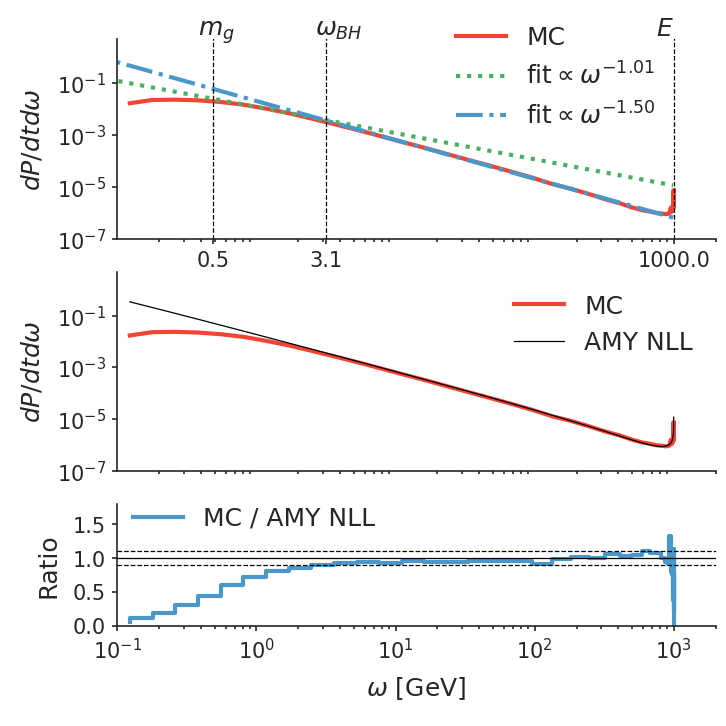
\includegraphics[width=\columnwidth]{spectrum.png}
\caption{The $q\rightarrow q+g$ splitting rate in an infinite medium from a quark with $E=1$ TeV,and a coupling constant $\alpha_s = 0.1$. The top plot shows the simulated spectrum $dR/d\omega$ (red-dashed line) and power law fit (green-dotted and blue-dash-dotted lines) in different gluon energy regions, separated by energy scales $\omega_{BH}\approx 2\pi T$. The middle plot compares to the simulation to NLL solution to the AMY equation, and the ratio is shown in the bottom plot}
\label{fig:spectrum}
\end{figure}

\begin{figure}
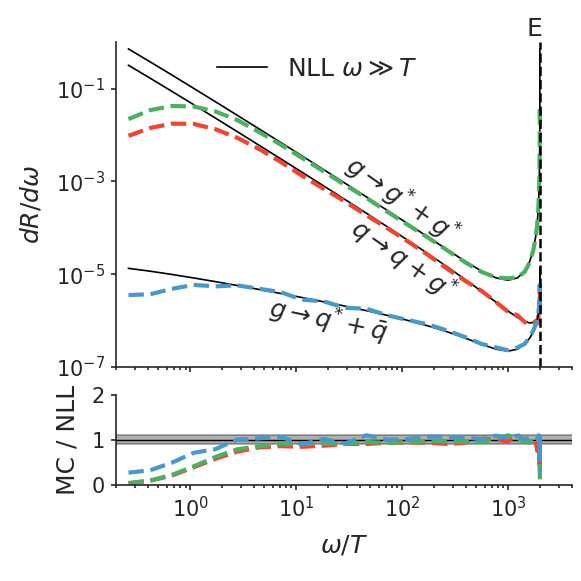
\includegraphics[width=\columnwidth]{channel_rate.png}
\caption{The splitting rate of $q\rightarrow q+g^*$, $g\rightarrow g+g^*$, and $g\rightarrow q^* + \bar{q}$ as a function of the parton energy labeled by the star. The mother parton with $E=1$ TeV evolves inside an infinite medium with $T=0.5$ GeV. The simulations (thick dashed lines) are compared to the NLL solutions (thin solid lines).}
\label{fig:channel_rate}
\end{figure}

\begin{figure}
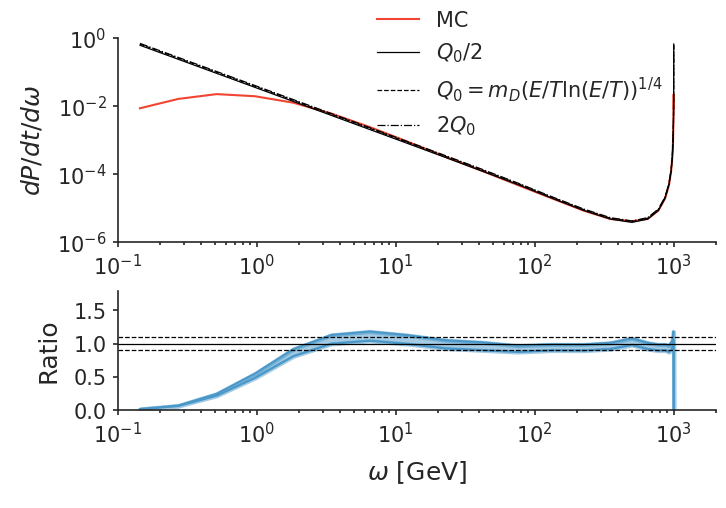
\includegraphics[width=\columnwidth]{running.png}
\caption{Top plot: comparison of modified Boltzmann simulation with the NLL solution  with running coupling.
Three initial guesses of the 
The ratio between simulation and theory is shown in the bottom plot.}
\label{fig:running}
\end{figure}

In this section, we compare the splitting rate $dR/d\omega$ that comes out of the modified Boltzmann approach simulation to the NLL approximation in the infinite medium limit.

The differential rate in an infinite medium $dR/d\omega$ is shown in Figure \ref{fig:spectrum} for a 1 TeV quark splitting into a gluon and a quark.
The temperature of the medium is $T=0.5$ GeV, and a rather small coupling constant $\alpha_s = 0.1$.
Please also refer to appendix \ref{app:tune-spectrum} for a full comparison varying both the parton energy and the coupling constant.
The horizontal axis is the radiated gluon energy.
In the upper plot, we divided the spectrum into different regions by the gluon thermal mass $m_\infty$ and an estimated Bethe-Heitler energy $\lambda_g m_D^2 \sim 2\pi T$.
The spectrum at $\omega < m_g$ is suppressed due the gluon thermal mass.
In the Bethe-Heitler region $\omega < 2\pi T$, the spectrum scales like $\omega^{-1}$ as given by the incoherent radiation rate.
In the deep LPM region $T \ll \omega < E$, the spectrum is dominated by coherent multiple scatterings and scales like $\omega^{-3/2}$.
The power-law fits in each domain are very close to the expected scaling.
In the middle plot, we compare the simulation to the NLL solution with self-consistent $Q_1^2$ from Eq. \ref{eq:Q1-sf}. 
The ratio between the two is shown in the bottom plot.
There is a good agreement in the LPM region between the simulation and the theory calculation, which we have used as guidance in developing our Monte-Carlo approach.

A comparison of the other channels $g\rightarrow g+g$ and $g\rightarrow q+\bar{q}$ to the theory calculations are shown in Figure \ref{fig:channel_rate}.
For the splitting parton energy much greater than temperature $\omega > 10 T$, the simulation agrees well with the NLL solution. 
Again, please also refer to appendix \ref{app:tune-spectrum} for comparison varying both $E$ and $\alpha_s$ for these two channels.


Finally, we compare the running coupling calculation with the theory curve in Fig. \ref{fig:running} for the $g\rightarrow g+g$ channel.
The theory curves (black lines) are obtained combining Eq. \ref{eq:AMY-LL} and Eq. \ref{eq:q3running}.
Different line styles correspond to the variation of the $Q_0$ value around an initial guess $m_D (E/T \ln(E/T) )^{1/4}$ by a factor of $2$ above and below.
For this 1 TeV parton, the scale $Q_0$ is actually very large and the running of $\alpha_s$ is rather slow, which explains the theory curve is not very sensitive to a factor of $4$ change in $Q_0$.
The simulation was performed using the running coupling prescription described in Section \ref{section:running}.
The overall shape of the spectrum in the deep LPM region is again well described by the modified Boltzmann simulation. 


\section{Towards phenomenological applications}\label{section:more}
In the previous section, we showed that the modified Boltzmann equation simulation has a good agreement with the theoretical calculation for parton splitting in the LPM regime in an infinite medium.
Towards future phenomenological application, we would like to investigate a few more complex scenarios involving a finite and expanding medium.

\subsection{A finite medium}
For calculation in a finite medium, there is an intricate interference pattern near the boundary which requires solving the original equation using a finite medium temperature profile. 
Or for the case of a thin medium, such effect can be analyzed order by order in the ``opacity ($L/\lambda$) expansion". 
One important effect in a finite medium is the path-length dependent radiation rate for $L \lesssim \tau_f$, which is important for heavy-ion collisions phenomenology, considering the formation time of very energetic splitting can be comparable to the size of the QGP fireball.
Though the modified Boltzmann approach has been constructed to mimic the rate $dR/d\omega$ in the infinite medium limit, and does not recover the exact form of spectrum for a finite medium, it still predicts an $L$-dependent rate and we would like to check whether it is significantly different from the theory expectation.
The origination of the path-length dependence in the modified Boltzmann approach is that the gluons sampled at $t=t_0$ are not considered as independent objects until $t = t_0+\tau_f$, meaning the splittings at time $t$ is initiated by inelastic processes at $t-\tau_f$.
As a result, in a semi-infinite medium with a step function like temperature profile, 
\begin{eqnarray}
T = \begin{cases}
0 , z<0\\
T_0, z>0
\end{cases}
\end{eqnarray}
there are no scattering centers at $L-\tau_f<0$ and thus introduces a reduction in the radiation rate for small path-length.

\begin{figure}
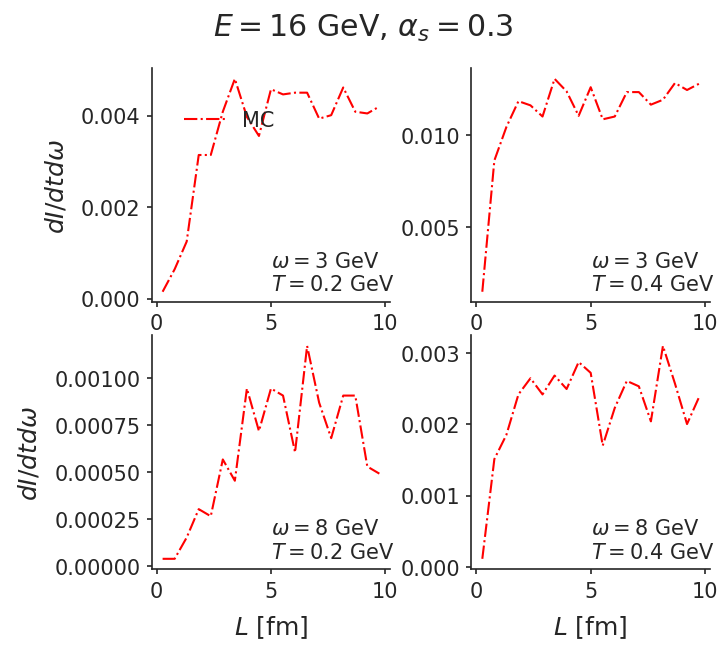
\includegraphics[width=\columnwidth]{spectrum_L.png}
\caption{Comparison of the path-length dependent rate $dR/d\omega$ from the simulation using $\alpha_s = 0.3$ to the theoretical calculation for splitting $q\rightarrow q+g$ \cite{CaronHuot:2010bp}. The quark energy is $16$ GeV.}
\label{fig:spectra-L-alphas=0.3}
\end{figure}

In Figure \ref{fig:spectra-L-alphas=0.3}, the $q\rightarrow q+g$ rate simulated in a semi-infinite medium is compared to the full calculations obtained in \cite{CaronHuot:2010bp}.
The energy of the quark is 16 GeV, and $\alpha_s = 0.3$.
The medium temperature of the left and the right columns are 0.2 GeV and 0.4 GeV respectively.
Top and bottom rows show the differential rates for the emitted gluon  energy $\omega = 3$ GeV and $\omega = 8$ GeV \footnote{In practical simulation, the rate are obtained by counting gluons within a finite energy range $\omega\pm 0.5$ GeV}.
The different rate $dR/d\omega$ are plotted as function of the path length $L$.
It is evident that theoretical rates (black solid lines) first grow approximately linearly with $L$ and then bend over to transit to $L$-independent ones.
The simulation describes the large $L$ limit well and also approximately captures the point at which the transition happens.
But there are systematic deviations compared to the theory at small path-length.
Therefore it will be of great interest to improve to the current simulation approach at small path-length in the future. 
For example, one possible solution would be using the results from the opacity expansion in the simulation for those splittings that happened close to the boundary and developing matching conditions to the approach we used for the deep LPM regime.

\subsection{An expanding medium}
\begin{figure}
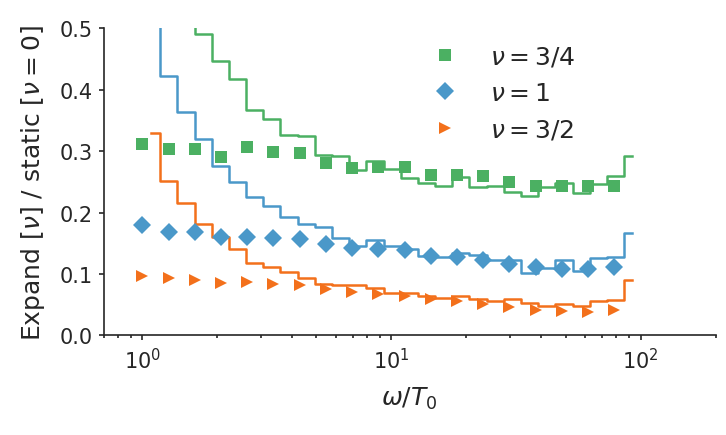
\includegraphics[width=\columnwidth]{spectrum_Bjorken.png}
\caption{The ratios of induced splitting rate in expanding medium to that of a stat medium, with expansion parameter $\nu = 3/4, 1$, and $3/2$. The analytic results are shown in solid lines and simulations denoted as symbols. The conpling constant $\alpha_s=0.3$, the expansion starts at $\tau_0 = 0.2$ fm/$c$ with an initial temperature $T_0 = 1$ GeV.}
\label{fig:Bjorken-BDMPS}
\end{figure}

The expansion of the medium is another important aspects for heavy-ion collision phenomenology.
The created QGP fireballs undergo dramatic expansion, causing the medium temperature at mid-rapidity to drop quickly in the first few fm$/c$.
This introduces another macroscopic scale in additional to the path length, which is the inverse medium expansion rate. 
In the context of this work, we shall define this expansion time scale as the inverse changing rate of $T^3$,
\begin{eqnarray}
\tau_{\textrm{ex}} = \left(\frac{d\ln(T^3)}{d \tau} \right)^{-1},
\end{eqnarray}
to be understood as the time scale over which the local $\hat{q}\propto T^3$ changes notably.
For simplicity, parametrize the temperature profile as a power law fall-off function of the proper time at mid-rapidity,
\begin{eqnarray}
T(\tau; \nu)^3 = T_0^3\left(\frac{\tau_0}{\tau}\right)^{2-1/\nu},
\end{eqnarray}
where the static case is recovered when $\nu=1/2$, and $\nu=1$ corresponds to the temperature profile of a Bjorken flow.
The resultant expansion time scale is
\begin{eqnarray}
\tau_{\textrm{ex}} = \frac{\tau}{2-1/\nu}.
\end{eqnarray}
If this time scale is smaller than the formation time of the splitting, then the medium cannot be well approximated by having a constant temperature when we resumes the multiple scatterings.
Fortunately, in the current modified Boltzmann approach, since we propagate the splitting process in real time, the fast changing of the medium temperature does affect the multiple scatterings that contribute to this specific splitting.

We would like to compare the response of the modified Boltzmann approach to an expanding medium to theoretical calculations.
The theoretical formula we used is obtained in the BDMPS framework 
by the authors of \cite{Baier:1998yf} using the power law type temperature profile. 
The total splitting probability is,
\begin{eqnarray}
\frac{dP}{d\omega} &=& \frac{\alpha_s}{2\pi E}P_{q\rightarrow qg}(x)\mathfrak{Re}\int_{\tau_0}^{\tau_0+L}\frac{dt_f}{t_f}\int_{\tau_0}^{t_f}\frac{dt_i}{t_i} \frac{1}{\nu^2}\\
\nonumber
&& \left.\left[ I_{\nu-1}(z_i)K_{\nu-1}(z_f)-I_{\nu-1}(z_f)K_{\nu-1}(z_i)\right]^{-2}\right|_{\omega}^{\omega=\infty},\\
z_{i,f} &=& 2i\nu \sqrt{\frac{\hat{q}_g(1-x+C_F/C_A x^2)}{2(1-x)\omega}} \tau_0 \left( \frac{t_{i,f}}{\tau_0}\right) ^{1/2\nu}
\end{eqnarray}
for the $q\rightarrow q+g$ splitting.
For $\nu=1/2$, this expression reduces to the static BDMPS result \cite{Baier:1996kr}. 

As a remark, the BDMPS calculation considers the multiple-soft limit of the collision kernel and therefore does not include the logarithm that comes from the perturbative tail $1/q_\perp^4$. 
Accordingly, we turn off the large-$Q$ matrix-element scatterings and only retain diffusion plus diffusion-induced radiation components in our simulation.
Besides, $b=0.75$ is used without the logarithmic correction factor in Eq. \ref{eq:NLL-b}, and the same $\hat{q}_g = m_D^2 C_A\alpha_s T$ are input to the theory and the simulation.
To suppress other difference in the simulation and the theory, instead of making direct comparison of the spectrum $dP/d\omega$ to the BDMPS result, we compare the ratio of the splitting probability in an expanding medium to that of a static medium
\begin{eqnarray}
R_\nu = \frac{dP(T=T(\tau;\nu))/d\omega}{dP(T=T_0)/d\omega}
\end{eqnarray}
between simulation and theory to focus on the response to a fast dropping temperature profile compared to the static case.

The medium expansion starts at $\tau_0=0.2$ fm/$c$ with $T_0=1$ GeV and stops at $\tau = 20$ fm/$c$.
We take four choices of the expansion rate $\nu = 1/2, 3/4, 1, 3/2$, corresponding to a static medium, a slowly expanding medium, Bjorken flow, and a faster-than-Bjorken expansion respectively.
The ratio $R_\nu$ from both theory and simulation are shown in Fig. \ref{fig:Bjorken-BDMPS} for a 100 GeV quark with $\alpha_s=0.3$.
Again, for $\omega/T \gg 1$, the simulation displays the expected decreasing of medium-induced radiation due to the dropping of temperature.
In the future, we are looking forward to making direct comparison to the solution of Eq. \ref{eq:full-theory} with both varying temperature and adding medium flow effects.

\section{Comparison with two other Monte-Carlo methods for medium-induced splittings}\label{section:compare}
Before we conclude this work, it is beneficial to compare the current implementation of the medium-induced splittings with two other Monte-Carlo approaches.
We will also summarize the features and caveats of these two methods for readers reference on this subject. 
Also, because the other two methods predicts very different radiation spectrum, it is not so instructive to compare their spectrum directly.
Instead, we compare the ``energy loss" of a quark from gluon radiation from between these approaches,
\begin{eqnarray}
\frac{dE}{dL} = \int \omega \frac{dR^q_{qg}}{d\omega} d\omega.
\label{eq:eloss}
\end{eqnarray}
As a remark, this definition is not related to the actually parton / jet energy loss in a medium, but only as a simply way to quantify the difference between different methods.
We shall see that due to different implementations of the medium-induced radiation, the amount of ``energy loss'' are very different between these approaches with the same $\alpha_s$.
As a result, an extraction of interested medium properties from experimental data using these models can be biased by the way they treat radiative processes.
Therefore, being able to calibrate a model to theoretical calculations as demonstrated in this work is an essential step prior to the comparison to experimental data.

\subsection{The approached used in the improved Langevin equation}
This approach is implemented in the improved Langevin equation \cite{Cao:2013ita}, using a higher-twist calculation of medium-induced single-gluon emission rate and a prescription to do multiple emission in a time-evolution manner.
The higher-twist formula for single radiation rate reads,
\begin{eqnarray}
\frac{dN_g}{dx dk_\perp^2 dt} = \frac{\alpha_s P(x)\hat{q}_g}{\pi k_\perp^4} 2\left(1-\cos\frac{t-t_0}{\tau_f}\right)
\end{eqnarray}
The rate is time-dependent, coming from the interference between the production of the hard parton at time $t_0$ and one interaction with the medium at time $t$.
From the second emission, the authors of \cite{Cao:2013ita} implements the following prescription: set the time $t_0$ to the time of the previous emission so that the probability of the next emission starts to accumulate from zero again as time increases.
Though it is not immediately clear what this prescription predicts without a simulation, it is possible to get a qualitative understanding by realizing that the typical time separation between two emissions of this model is a time scale $\Delta t = t-t_0$ within which the emission probability is of order one,
\begin{eqnarray}
1 \sim \int_{t_0}^{t} dt\int_{x_c}^1 dx \int dk_\perp^2 \frac{dN_g(t-t_0)}{dx dk_\perp^2 dt}.
\end{eqnarray}
In the soft limit where $P(x) \sim 2/x$, $\tau_f\sim 2xE/k_\perp^2$, and perform the time integral first, then the $k_\perp$ integral with limits from $0$ to $xE$.
The $x$ (with a change of variable to $u = xE\Delta t/2$) integral here divergent at 0.
Though this is not a problem for energy loss, had one also included the absorption processes according to detailed balance.
But for this prescriptions replies on the rate, we have to render the integral finite with a minimum cut-off $x_c$
\begin{eqnarray}
1 &\sim& 4\alpha_s\hat{q}\Delta t \int_{x_c}^1 \frac{dx}{x} \int \frac{dk_\perp^2}{k_\perp^4}\left(1-\frac{\sin(\Delta t/\tau_f)}{\Delta t/\tau_f}\right)\\
&=& \frac{\alpha_s\hat{q}_g \Delta t^3}{3u^3} \left( u^3\mathrm{Ci}(u)-3u^2\mathrm{Si}(u) - u^2 \sin(u) \right. \\\nonumber
&&\left. +3u-\sin(u) - 2u\cos(u) \right) \left.\right|_{\frac{\Delta t E x_c}{2}}^{\frac{\Delta t E}{2}} 
\end{eqnarray}
The result can be expanded at small $u$: $\frac{1}{18}(6\ln(u)+6\gamma_E - 17)$, besides it decays to $0$ at infinity, so a good proxy is to use the small-$u$ expansion but cut-off the upper bound at its zero,
\begin{eqnarray}
1 &\sim&  \frac{\alpha_s\hat{q}\Delta t^3}{3}\ln\frac{2}{ x_c E \Delta t } \propto (g^2 T \Delta t)^3 \ln\frac{2}{ x_c E \Delta t }.
\label{eq:delta-t-formula}
\end{eqnarray}
One sees that typical time between two emissions in this approach is on the order of $1/g^2T$ which the same as the elastic mean-free-path.
Putting typical $\Delta t \sim \lambda_{el}$ back to the factor $2(1-\cos(\Delta t/\tau_f))$, the radiation spectrum is indeed suppressed when $\tau_f \gg \lambda_{el}$.
However, this suppression is introduced by controlling the correlation between two subsequent emissions, while the LPM suppression actually happens on the level of single emission rate.
Moreover, the logarithmic factor in equation \ref{eq:delta-t-formula} depends on the infrared cut-off (in the original work, this cut-off is chosen at $\pi T$), therefore the prediction can be cut-off dependent, though logarithmic slow.
This is due to that this correlation prescription changes the second emission rate in the same way, no matter how soft the previous emission is.
This is in fact a feature we want to avoid.

\subsection{The ``blocking radiation'' approach}
Another method \cite{ColemanSmith:2012vr} will be termed as the ``blocking radiation approach" in this work.
In this approach, the splitting is also first generated through an incoherent process at time $t_0$, then followed by a self-consistent determination of formation time with elastic broadening.
These steps are the same as the modified Boltzmann approach in this work.
However, the LPM suppression is introduced by requiring no additional radiation is allowed during the formation time of the previous one. 
This is different form this work, where the emitter can have an arbitrary number of independent ``pre-formed'' splitting copies.
Again, this ``blocking radiation'' approach introduces correlations between subsequent emissions.
A closer investigation reveals bigger problem.
In an infinite medium, this approach reduces every $\tau_f/\lambda_{inel}$ incoherent emission to one, resulting only an overall reduction in the radiation spectrum without changing its shape.
And the suppression factor $\lambda_{inel}/\tau_f$ is a comparison between  the formation time with the incoherent inelastic mean-free-path, instead of the elastic mean-free-path, which is off by a power of $\alpha_s$.

\begin{figure*}
\centering
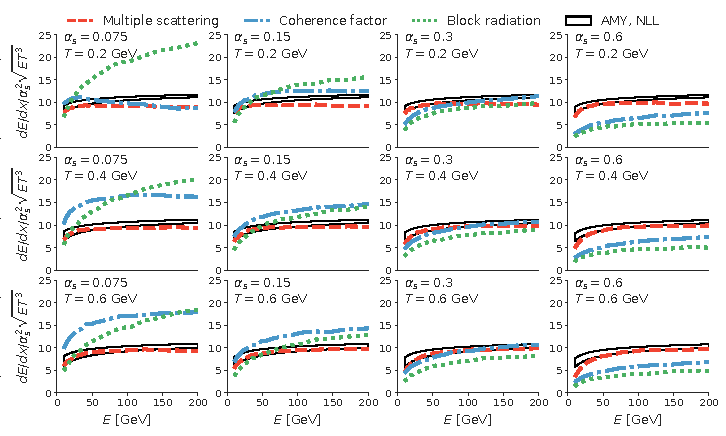
\includegraphics[width=1.\textwidth]{Eloss_infinite.pdf}
\caption{Energy loss per unit path lengh $dE/dL$ as a function of energy $E$, temperature $T$ and coupling constant $\alpha_s$. Each column corresponds to a value of the coupling constant $\alpha_s = 0.075, 0.15, 0.3$, and $0.6$ (from left to right). Each row corresponds to a temperature of $T = 0.2, 0.4$, and $0.6$ GeV (from top to bottom). $dE/dx$ is divided by the expected scaling $\alpha_s^2 \sqrt{ET^3}$. The MC implementations of the LPM effect referred to as ``modified Boltzmann", ``coherence factor", and ``blocking radiation" approaches are shown with red-dashed lines, blue-dash-dotted lines, and green-dotted lines respectively. The AMY NLL results are denoted as black boxes.}
\label{fig:eloss-inf}
\end{figure*}


\subsection{Comparison with the modified Boltzmann approach and the analytic results}
In Figure \ref{fig:eloss-inf}, we show the calculation of ``energy loss'' defined in \ref{eq:eloss} of a quark in an ``infinitely large" medium. 
The results presented are normalized by $1/(\alpha_s^2 \sqrt{ET^3})$ in anticipation of the scaling $dE/dx \propto \alpha_s^2 \sqrt{ET^3}$.
For each column, we double the value of $\alpha_s$ and for each row, the temperature is increased by $0.2$ GeV. 
Within each subplot, the parton energy varies from $10$ GeV to $200$ GeV.
The three Monte-Carlo methods of medium-induced energy loss are shown in colored lines, 
NLL AMY results are shown as black lines where we only integrate $\omega$ above the the Debye mass.
As expected, the modified Boltzmann approach (red-dashed lines) which describes the radiation spectrum also reproduces the energy, temperature, and coupling constant dependence of the energy loss.
The method used in the improved-Langevin equation (blue-dash-dotted lines) has a similar energy and temperature dependence as the theoretical baseline; however, it systematically deviates from the baseline for different values of the coupling constant in a logarithmic manner.
For the ``block radiation" approaches, the deviations from the baseline regarding their $\alpha_s$-dependence is completely off, which is not surprising as we have discussed its shortcomings.


\section{Summary and outlook}\label{section:summary}
We have investigated the modification to the incoherent Boltzmann transport approach to include the LPM effect for parton splitting processes in the deep LPM region, with the guidance from the LL and the NLL solutions of the AMY equation.
The running coupling effect has also been implemented in this approach.
The overall level of agreement between the simulated results and theoretical calculations in the infinite medium limit is promising given the simplicity of this Monte-Carlo procedure. 
Although it was developed for the deep LPM regime, the current approach captures qualitative features of the path-length dependence of medium induced splittings and the qualitative change of the spectrum shape in an expanding medium compared to the static case.
Of course, it is important to improve this method for the case of a thin medium.
Another interest of study would be a consistent inclusion of the heavy quark mass effect into the current approach.
We shall seek for improvements in these aspects in future works.

Being able to calibrate a Monte-Carlo transport model to theoretical calculation is important.
As we have argued in section \ref{section:compare}, different modeling of the medium-induced radiation can bias the extraction of the medium properties (such as the interaction strength).
The design of this modified Boltzmann transport approach and its systematic comparison to theoretical calculations allow us to reduce and estimate the uncertainty in these implementations.
This is instrumental for performing an examination of theory assumptions and a more meaningful phenomenological extraction of jet transport properties from future model-to-data comparison in transport model based studies.

\begin{acknowledgments}
SAB, WK and YX are supported by the U.S. Department of Energy Grant no. DE-FG02-05ER41367. WK is also supported by NSF grant OAC-1550225.
WK would like to thank Florian Senzel, Jean-Francois Paquet and Yacine Mehtar-Tani for helpful discussions.
\end{acknowledgments}

\begin{appendices}
\section{Approximation of the $2\rightarrow 3$ matrix-elements}
\label{app:23}
Regarding the $2\rightarrow 3$ matrix-element, in previous study \cite{Ke:2018tsh}, we used to employ an improved version of the original Gunion-Bertsch cross-section that works under the limits $k_\perp, q_\perp \ll \sqrt{s}$ and $x q_\perp \ll k_\perp$ \cite{PhysRevD.25.746,Fochler:2013epa,Uphoff:2014hza}.
The original Gunion-Bertsch cross-section \cite{PhysRevD.25.746} only works for soft emissions $x=k^+/p^+ \ll 1$. 
With the improvements made in \cite{Fochler:2013epa,Uphoff:2014hza}, the agreement with the exact matrix-elements is extended to large-$x$, but still the splitting function is only reproduced to $O(x)$.
In the present study, we relax the condition $x q_\perp \ll k_\perp$ in the derivation, so that the full leading order vacuum splitting function can be recovered.
We summarize the matrix-elements here,
\begin{eqnarray}
\overline{|M^2|}_{g+i\rightarrow g+g+i} &=& \overline{|M^2|}_{g+i\rightarrow g+i} P_{gg}^{g(0)}  D_{gg}^{g},\\
\overline{|M^2|}_{g+i\rightarrow q+\bar{q}+i} &=& \frac{C_F d_F}{C_A d_A}\overline{|M^2|}_{g+i\rightarrow g+i} P_{q\bar{q}}^{g(0)} D_{q\bar{q}}^{g},\\
\overline{|M^2|}_{q+i\rightarrow q+g+i} &=& \overline{|M^2|}_{q+i\rightarrow q+i} P_{qg}^{q(0)} D_{qg}^{q},
\end{eqnarray}
where $\overline{|M^2|}_{g+i\rightarrow g+i}$, $\overline{|M^2|}_{g+i\rightarrow g+i}$ and $\overline{|M^2|}_{q+i\rightarrow q+g+i}$ are the spin-color averaged two-body collision matrix-elements with only $\hat{t}$-channel contribution.
Index $i$ represent a medium quark / anti-quark or a medium luon.
The $P_{bc}^{a(0)}(x)$ terms are vacuum splitting functions of parton $a$ to partons $b$ and $c$. 
\begin{eqnarray}
P_{gg}^{g(0)}  &=& g^2  C_A\frac{1+x^4+(1-x)^4}{x(1-x)},\\
P_{qg}^{q(0)} &=& g^2  C_F\frac{1+(1-x)^4}{x},\\
P_{q\bar{q}}^{g(0)} &=& g^2  \frac{N_f}{2}\left(x^2+(1-x)^4\right).
\end{eqnarray}
Finally, the $D_{bc}^{a}$ terms are,
\begin{eqnarray}
D_{qq}^{g} &=& 
C_A(\vec{a}-\vec{b})^2 + C_A(\vec{a}-\vec{b})^2 \\\nonumber
&-& C_A (\vec{a}-\vec{b})\cdot (\vec{a}-\vec{c}),
\\
D_{q\bar{q}}^{g} &=& 
C_F(\vec{a}-\vec{b})^2 + C_F(\vec{a}-\vec{b})^2 \\\nonumber
&-& (2C_F-C_A) (\vec{a}-\vec{b})\cdot (\vec{a}-\vec{b}),
\\
D_{qg}^{q} &=& 
C_F(\vec{c}-\vec{a})^2 + C_F(\vec{c}-\vec{b})^2 \\\nonumber
&-& (2C_F-C_A) (\vec{c}-\vec{a})\cdot (\vec{c}-\vec{b}),
\end{eqnarray}
with the vectors given by
\begin{eqnarray}
\vec{a} = \frac{\vec{k}_\perp - x\vec{q}_\perp}{(\vec{k}_\perp - x\vec{q}_\perp)^2};
\vec{b} = \frac{\vec{k}_\perp - \vec{q}_\perp}{(\vec{k}_\perp - \vec{q}_\perp)^2};
\vec{c} =  \frac{\vec{k}_\perp}{\vec{k}_\perp^2}.
\end{eqnarray}

\begin{figure}
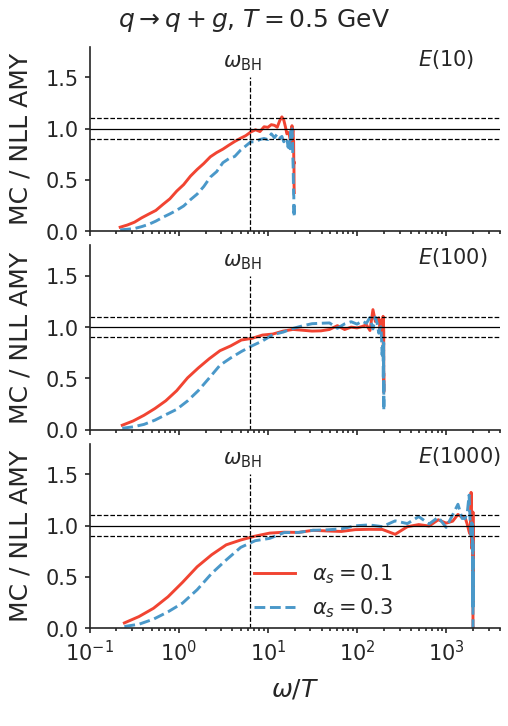
\includegraphics[width=\columnwidth]{spectrum_E_q2qg.png}
\caption{Ratios of splitting rate $dR/\omega$ between the modified Boltzmann simulation and the NLL solution for $q\rightarrow q+g$ splitting. The quark energies are $E$ is 10, 100, and 100 GeV from top to the bottom plot. 
And two coupling constants are used: $\alpha_s = 0.1$ (red solid lines) and $\alpha_s = 0.3$ (blue dashed lines).
$\omega$ stands for the gluon energy.
The horizontal dashed lines denote $\pm 10\%$ deviation from unity. }
\label{fig:q2qg}
\end{figure}

\begin{figure}
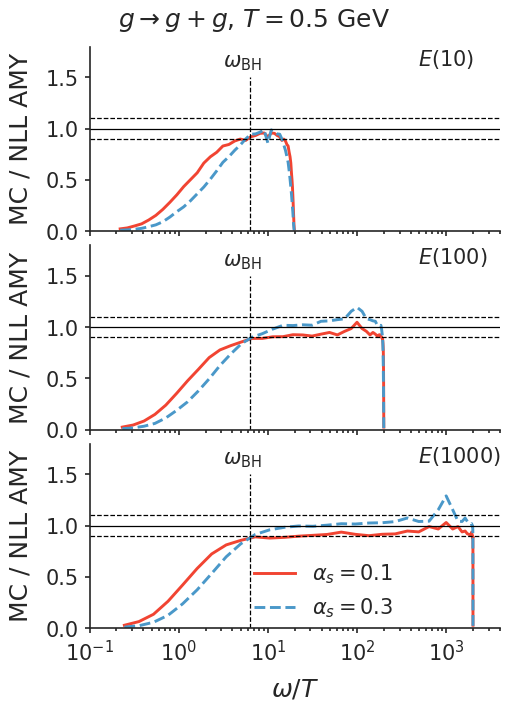
\includegraphics[width=\columnwidth]{spectrum_E_g2gg.png}
\caption{The same as Fig. \ref{fig:g2gg}, but for the $g\rightarrow g+g$ splitting, and $\omega$ stands for either energy of the final state gluon.}
\label{fig:g2gg}
\end{figure}

\begin{figure}
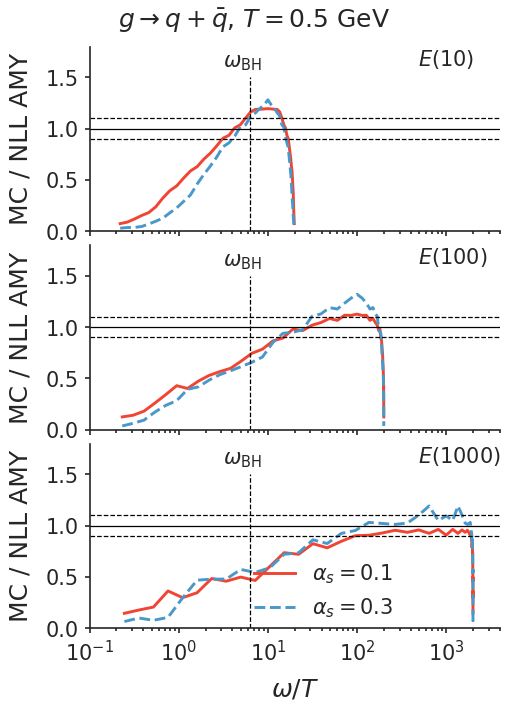
\includegraphics[width=\columnwidth]{spectrum_E_g2qqbar.png}
\caption{The same as Fig. \ref{fig:g2gg}, but for the $g\rightarrow q+\bar{q}$ splitting, and $\omega$ stands the energy of the quark.}
\label{fig:g2qqbar}
\end{figure}

\section{Energy and coupling constant dependence of the splitting rate}
\label{app:tune-spectrum}
In this appendix, we provide comparisons of splitting rate at different values of energy and coupling constant for the reader's references.
Fig. \ref{fig:q2qg}, Fig. \ref{fig:g2gg} and Fig. \ref{fig:g2qqbar} shows the comparison for channels $q\rightarrow q+g$, $g\rightarrow g+g$ and $g\rightarrow q+\bar{q}$ respectively.
The results are shown as the ratio between the simulations and the NLL solution.
Within in each figure, the mother parton energy are 10 GeV, 100 GeV and 1000 GeV from the top to bottom plot.
We have used two coupling constants at $\alpha_s = 0.1$ (red solid lines) and $\alpha_s = 0.3$ (blue dashed lines).

\end{appendices}
\bibliography{mclpm} 
\end{document}
